\documentclass[nooutcomes]{ximera}
%% handout
%% space
%% newpage
%% numbers
%% nooutcomes

%I added the commands here so that I would't have to keep looking them up
%\newcommand{\RR}{\mathbb R}
%\renewcommand{\d}{\,d}
%\newcommand{\dd}[2][]{\frac{d #1}{d #2}}
%\renewcommand{\l}{\ell}
%\newcommand{\ddx}{\frac{d}{dx}}
%\everymath{\displaystyle}
%\newcommand{\dfn}{\textbf}
%\newcommand{\eval}[1]{\bigg[ #1 \bigg]}


\newcommand{\RR}{\mathbb R}
\renewcommand{\d}{\,d}
\newcommand{\dd}[2][]{\frac{d #1}{d #2}}
\renewcommand{\l}{\ell}
\newcommand{\ddx}{\frac{d}{dx}}
\newcommand{\dfn}{\textbf}
\newcommand{\eval}[1]{\bigg[ #1 \bigg]}

\usepackage{multicol}

\renewenvironment{freeResponse}{
\ifhandout\setbox0\vbox\bgroup\else
\begin{trivlist}\item[\hskip \labelsep\bfseries Solution:\hspace{2ex}]
\fi}
{\ifhandout\egroup\else
\end{trivlist}
\fi} %% we can turn off input when making a master document

\title{3.7 The Chain Rule (Solutions)}  

\begin{document}
\begin{abstract}		\end{abstract}
\maketitle

\section*{Warm up:} 
True or False:
	\begin{enumerate}[label=\Roman*.]
	
	\item  The function $e^{7x^2}$ can be differentiated without using the Chain Rule.
		\begin{freeResponse}
		False.  $\ddx \left( e^{7x^2} \right) = e^{7x^2} \cdot \ddx \left( 7x^2 \right) = 14x e^{7x^2}$.  
		\end{freeResponse}	
		
	\item  The derivative of a product is not the product of the derivatives.  But the derivative of a composition is a product of derivatives.
		\begin{freeResponse}
		True!
		
		$\ddx (f(x) g(x)) = f'(x) g(x) + f(x) g'(x)$.
		
		$\ddx(f(g(x))) = f'(g(x)) \cdot g'(x)$.
		\end{freeResponse}	
		
	\end{enumerate}
	
	
	
	
	

\section*{Group work:}



%problem 1
\begin{problem}
Differentiate each function (with respect to $x$)

	\begin{enumerate}
	
	%part a
	\item  $\cos \left( \sqrt{x+7} \right) $
		\begin{freeResponse}
		\begin{align*}
		\ddx \left( \cos \left( \sqrt{x+7} \right) \right) &= -\sin \left( \sqrt{x+7} \right) \cdot \frac{1}{2} (x+7)^{\frac{-1}{2}} (1) \\
		&= \frac{-\sin \left( \sqrt{x+7} \right) }{2 \sqrt{x+7}}
		\end{align*}
		\end{freeResponse}
		
		
		
	%part b
	\item  $\sqrt{ \cos x + 7}$
		\begin{freeResponse}
		\begin{align*}
		\ddx \left( \sqrt{ \cos x + 7} \right) &= \frac{1}{2} \left( \cos x + 7 \right)^{\frac{-1}{2}} \left( -\sin x \right) \\
		&= \frac{- \sin x }{2 \sqrt{\cos x + 7 }}
		\end{align*}
		\end{freeResponse}
		
		
		
	%part c
	\item $\sqrt{\cos x} + 7$
		\begin{freeResponse}
		\begin{align*}
		\ddx \left( \sqrt{\cos x} + 7 \right) &=  \frac{1}{2} \left( \cos x \right)^{\frac{-1}{2}} \left( -\sin x \right) + 0  \\
		&= \frac{- \sin x}{2 \sqrt{\cos x}}
		\end{align*}
		\end{freeResponse}
		
		
		
	%part d
	\item  $\cos \left( \sqrt{x} + 7 \right)$
		\begin{freeResponse}
		\begin{align*}
		\ddx \left( \cos \left( \sqrt{x} + 7 \right) \right) &= - \sin \left( \sqrt{x} + 7 \right) \cdot \frac{1}{2} x^{\frac{-1}{2}} \\
		&=  \frac{- \sin \left( \sqrt{x} + 7 \right) }{2 \sqrt{x}}
		\end{align*}
		\end{freeResponse}
		
		
		
	\end{enumerate}
			
			
	
\end{problem}
















%problem 2
\begin{problem}
For the following problems, the derivative is given.  Determine which function was the original function.
	\begin{enumerate}[label=\roman*.]
	
		\item  The derivative is $f'(x) = \cos (x) e^{\sin x}$.  Which is the original function?
		
			\begin{enumerate}
			
			\item  $f(x) = (\sin x)(e^x)$
			\item  $f(x) = \sin (e^x)$
			\item  $f(x) = e^{\sin x}$
			\item  $f(x) = e^{x \sin x}$
			
				\begin{freeResponse}
				Since
				$$ \ddx \left( e^{\sin x} \right) = e^{\sin x} \cdot \cos x = \cos(x) e^{\sin x} $$
				the correct answer is (c).  
				\end{freeResponse}
				
			\end{enumerate}
			
			
			
		\item  The derivative is $g'(x) = 4 \left( \tan (x^4 - 5x) \right)^3 \sec^2(x^4-5x)(4x^3-5)$.  Which is the original function?
		
			\begin{enumerate}
			
			\item  $g(x) = \left( \tan x - 5x \right)^4$
			\item  $g(x) = \tan^4x - 5x^4$
			\item  $g(x) = \tan(x^4 - 5x)$
			\item  $g(x) = \tan^4(x^4-5x)$
			
				\begin{freeResponse}
				Since 
				$$\ddx \left( \tan^4(x^4-5x) \right) = 4 \tan^3(x^4-5x) \sec^2(x^4-5x) (4x^3-5)$$ 
				the correct answer is (d).  Notice that $\tan^3(x^4-5x) = \left( \tan(x^4-5x) \right)^3$ are (slightly) different notations for the exact same expression.
				\end{freeResponse}
				
			\end{enumerate}
			
	\end{enumerate}
			
			
			
		
\end{problem}
	
	
	
	
	
	
	
	
			
			

%problem 3			
\begin{problem}
Suppose the line tangent to the graph of $f(x)$ at $x=1$ is $y=6x-7$.  Find an equation of the line tangent to the following curves at $x=1$:
	\begin{enumerate}
	
	%part a
	\item  $g(x) = 5(f(x))^4$  
		\begin{freeResponse}
		First, in the equation of the tangent line to $f(x)$ at $x=1$, when $x=1$ we have that $y= 6(1) - 7 = -1$.  Thus $f(1) = -1$ and therefore $g(1) = 5(-1)^4 = 5$.  Hence, a point on our line is $(1,5)$.  Also, since the slope of this tangent line is $m=6$, we know that $f'(1) = 6$.
		
		Now, by the chain rule we have that $g'(x) = 5 \cdot 4 (f(x))^3 \cdot f'(x)$.  So $g'(1) = 20(f(1))^3 \cdot f'(1) = 20(-1)^3 (6) = -120.$  Thus, the equation of the line tangent to the graph of $y = g(x)$ at $x=1$ is
		$$ y - 5 = -120(x-1) $$
		$$ y = -120x + 125 $$
		\end{freeResponse}
		
		
		
	%part b
	\item  $h(x) = x^2 (f(x^3))$
		\begin{freeResponse}
		$h(1) = 1^2 \cdot f(1^3) = f(1) = -1$.  By the product and chain rules:
		$$ h'(x) = 2x(f(x^3)) + x^2(f'(x^3) \cdot 3x^2) = 2x(f(x^3)) + 3x^4(f'(x^3)) $$
		Thus, $h'(1) = 2f(1) + 3f'(1) = 2(-1) + 3(6) = -2 + 18 = 16$.  So, the equation of the line tangent to the graph of $y=h(x)$ at $x=1$ is
		$$ y- (-1) = 16(x-1) $$
		$$ y = 16x - 17 $$
		\end{freeResponse}
		
		
		
	\end{enumerate}
		
		
		
	
		
\end{problem}









%problem 4			
\begin{problem}
Given the following graphs of $f(x)$ and $g(x)$ (both piecewise linear functions), define new functions $u(x) = f(g(x))$ and $v(x) = f(x)g(x)$.  Find:

\begin{image}
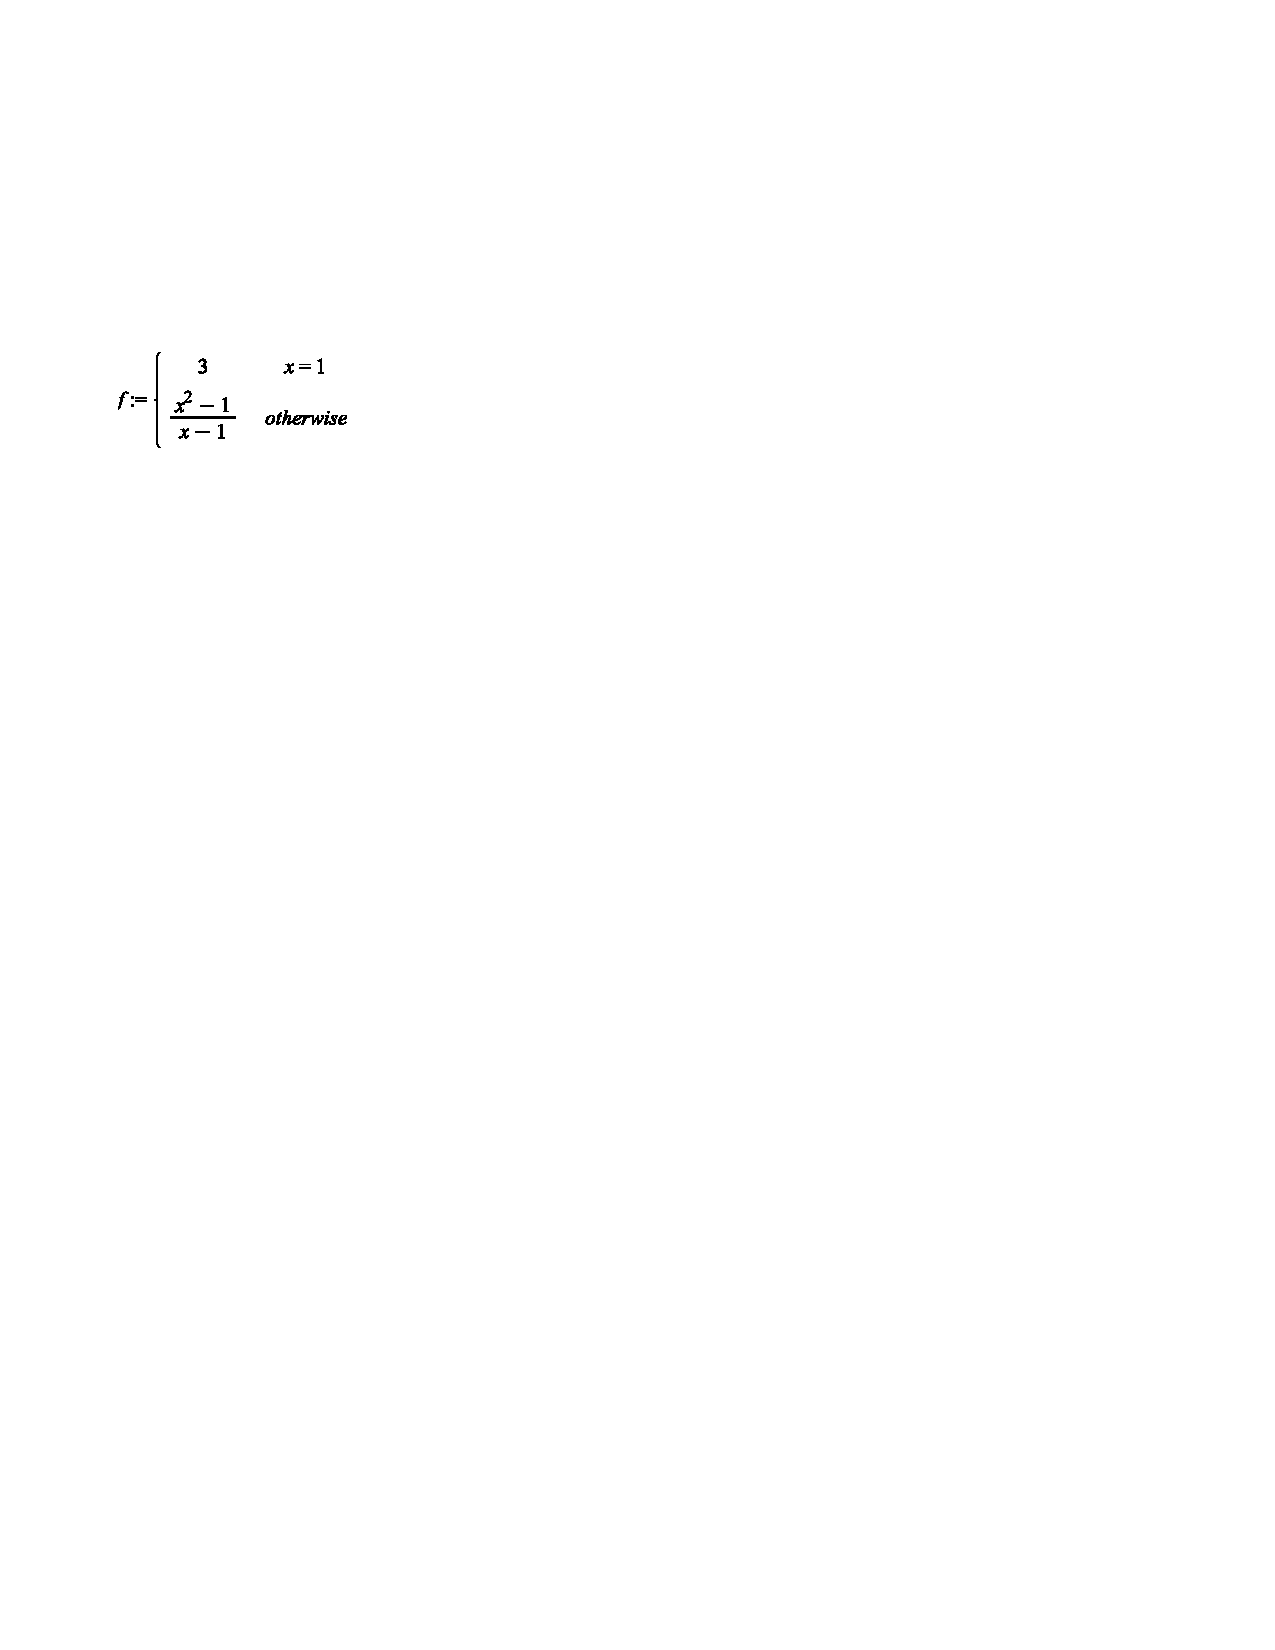
\includegraphics[trim= 170 420 250 230]{Figure7.pdf}
\end{image}

	\begin{enumerate}
	
	\item	$u'(1)$
		\begin{freeResponse}
		$u'(x) = \ddx(f(g(x))) = f'(g(x)) \cdot g'(x)$.  So, 
		\begin{align*}
		u'(1) &= f'(g(1)) \cdot g'(1) \\
		&= f'(1) \cdot (-1) \\
		&= (2)(-1) = -2 
		\end{align*}  
		\end{freeResponse}
		
		
		
	
	\item	$v'(1)$
		\begin{freeResponse}
		$v'(x) = \ddx(f(x)g(x)) = f'(x)g(x) + f(x)g'(x)$.  So,
		\begin{align*}
		v'(1) &= f'(1) g(1) + f(1) g'(1) \\
		&= (2)(1) + (2)(-1) \\
		&= 0
		\end{align*}
		\end{freeResponse}
		
		
		
	\end{enumerate}
		
		
		
	
		
\end{problem}







	
	
	
	
	
	
	
	
	

	










								
				
				
	














\end{document} 


















